Loading initial resources:

\begin{Shaded}
\begin{Highlighting}[]
\CommentTok{# Data manipulation}
\KeywordTok{library}\NormalTok{(tidyverse)}
\KeywordTok{library}\NormalTok{(magrittr)}

\CommentTok{# Utils}
\KeywordTok{library}\NormalTok{(neurotransmissionevolution)}

\CommentTok{# Packaged data}
\KeywordTok{data}\NormalTok{(}
\NormalTok{   cogs}
\NormalTok{  ,gene_ids}
\NormalTok{  ,gene_cogs}
\NormalTok{  ,string_eukaryotes}
\NormalTok{  ,}\DataTypeTok{package =} \StringTok{"neurotransmissionevolution"}
\NormalTok{)}

\CommentTok{# Fresh analysis data}
\NormalTok{cog_roots                   <-}\StringTok{ }\KeywordTok{read_tsv}\NormalTok{(}\StringTok{"geneplast_roots.tsv"}\NormalTok{,             }\DataTypeTok{col_types =} \StringTok{"ci"}\NormalTok{)}
\NormalTok{clade_names                 <-}\StringTok{ }\KeywordTok{read_tsv}\NormalTok{(}\StringTok{"geneplast_clade_names.tsv"}\NormalTok{,       }\DataTypeTok{col_types =} \StringTok{"ic"}\NormalTok{)}
\NormalTok{clade_taxids                <-}\StringTok{ }\KeywordTok{read_tsv}\NormalTok{(}\StringTok{"geneplast_clade_taxids.tsv"}\NormalTok{,      }\DataTypeTok{col_types =} \StringTok{"ici"}\NormalTok{)}

\CommentTok{# Collapsing similar functions}
\NormalTok{gene_annotation <-}\StringTok{ }\KeywordTok{read_tsv}\NormalTok{(}\StringTok{"../data/gene_annotation.tsv"}\NormalTok{, }\DataTypeTok{col_types =} \StringTok{"cc"}\NormalTok{) }\OperatorTok
\StringTok{  }\KeywordTok{mutate}\NormalTok{(}\DataTypeTok{annotation =} \KeywordTok{case_when}\NormalTok{(}
     \KeywordTok{grepl}\NormalTok{(}\StringTok{"clearance"}\NormalTok{,   annotation) }\OperatorTok{~}\StringTok{ "depletion"}
\NormalTok{    ,}\KeywordTok{grepl}\NormalTok{(}\StringTok{"degradation"}\NormalTok{, annotation) }\OperatorTok{~}\StringTok{ "depletion"}
\NormalTok{    ,}\KeywordTok{grepl}\NormalTok{(}\StringTok{"transport"}\NormalTok{,   annotation) }\OperatorTok{~}\StringTok{ "synthesis"}
\NormalTok{    ,}\OtherTok{TRUE} \OperatorTok{~}\StringTok{ }\NormalTok{annotation}
\NormalTok{  ))}
\end{Highlighting}
\end{Shaded}

A

\begin{Shaded}
\begin{Highlighting}[]
\CommentTok{# If a gene has more than 1 COG, select the oldest one.}
\CommentTok{# This is unusual, but can happen in cases of gene fusion, for instance.}
\NormalTok{gene_cogs }\OperatorTok
\StringTok{  }\KeywordTok{inner_join}\NormalTok{(cog_roots) }\OperatorTok
\StringTok{  }\KeywordTok{group_by}\NormalTok{(string_id) }\OperatorTok
\StringTok{  }\KeywordTok{filter}\NormalTok{(root }\OperatorTok{==}\StringTok{ }\KeywordTok{max}\NormalTok{(root))}

\CommentTok{# The function of a COG is the function of its proteins}
\NormalTok{cog_annotation <-}\StringTok{ }\NormalTok{gene_ids }\OperatorTok
\StringTok{  }\KeywordTok{inner_join}\NormalTok{(gene_cogs) }\OperatorTok
\StringTok{  }\KeywordTok{inner_join}\NormalTok{(gene_annotation) }\OperatorTok
\StringTok{  }\KeywordTok{distinct}\NormalTok{(cog_id, annotation)}

\CommentTok{# Number of proteins in a COG in every species}
\NormalTok{cog_size_by_taxid <-}\StringTok{ }\NormalTok{cogs }\OperatorTok
\StringTok{  }\KeywordTok{filter}\NormalTok{(cog_id }\OperatorTok\StringTok{ }\NormalTok{gene_cogs[[}\StringTok{"cog_id"}\NormalTok{]]) }\OperatorTok
\StringTok{  }\KeywordTok{count}\NormalTok{(taxid, cog_id, }\DataTypeTok{name =} \StringTok{"cog_size"}\NormalTok{)}

\CommentTok{# Number of COGs in every species}
\NormalTok{cog_n_by_taxid <-}\StringTok{ }\NormalTok{cog_size_by_taxid }\OperatorTok
\StringTok{  }\KeywordTok{count}\NormalTok{(taxid, }\DataTypeTok{name =} \StringTok{"cog_n"}\NormalTok{)}

\CommentTok{# Number of proteins in every species}
\NormalTok{protein_n_by_taxid <-}\StringTok{ }\NormalTok{cog_size_by_taxid }\OperatorTok
\StringTok{  }\KeywordTok{count}\NormalTok{(taxid, }\DataTypeTok{wt =}\NormalTok{ cog_size, }\DataTypeTok{name =} \StringTok{"protein_n"}\NormalTok{)}

\CommentTok{# Mapping species to clade info}
\NormalTok{ordered_species <-}\StringTok{ }\NormalTok{string_eukaryotes }\OperatorTok
\StringTok{  }\KeywordTok{select}\NormalTok{(taxid, ncbi_name) }\OperatorTok
\StringTok{  }\KeywordTok{left_join}\NormalTok{(clade_taxids) }\OperatorTok
\StringTok{  }\KeywordTok{left_join}\NormalTok{(clade_names, }\DataTypeTok{by =} \KeywordTok{c}\NormalTok{(}\StringTok{"lca"}\NormalTok{ =}\StringTok{ "root"}\NormalTok{)) }\OperatorTok
\StringTok{  }\KeywordTok{mutate}\NormalTok{(}
     \DataTypeTok{lca        =} \KeywordTok{as_factor}\NormalTok{(lca) }\OperatorTok\StringTok{ }\NormalTok{fct_rev}
\NormalTok{    ,}\DataTypeTok{ncbi_name  =} \KeywordTok{fct_reorder}\NormalTok{(ncbi_name, }\OperatorTok{-}\NormalTok{taxid_order)}
\NormalTok{    ,}\DataTypeTok{clade_name =} \KeywordTok{fct_reorder}\NormalTok{(clade_name, }\OperatorTok{-}\NormalTok{taxid_order)}
\NormalTok{  )}

\NormalTok{annotation_colors <-}\StringTok{ }\KeywordTok{c}\NormalTok{(}
   \StringTok{"depletion"}\NormalTok{             =}\StringTok{ "#F40000"}
\NormalTok{  ,}\StringTok{"excitability"}\NormalTok{          =}\StringTok{ "#FFAB00"}
\NormalTok{  ,}\StringTok{"receptor-associated"}\NormalTok{   =}\StringTok{ "#D6EE00"}
\NormalTok{  ,}\StringTok{"ionotropic receptor"}\NormalTok{   =}\StringTok{ "#43FF1C"}
\NormalTok{  ,}\StringTok{"metabotropic receptor"}\NormalTok{ =}\StringTok{ "#18FFFF"}
\NormalTok{  ,}\StringTok{"signaling"}\NormalTok{             =}\StringTok{ "#0091EA"}
\NormalTok{  ,}\StringTok{"g-protein"}\NormalTok{             =}\StringTok{ "#0033ff"}
\NormalTok{  ,}\StringTok{"synthesis"}\NormalTok{             =}\StringTok{ "#AA00FF"}
\NormalTok{  ,}\StringTok{"vesicle"}\NormalTok{               =}\StringTok{ "#FF00AA"}
\NormalTok{)}
\end{Highlighting}
\end{Shaded}

\begin{Shaded}
\begin{Highlighting}[]
\NormalTok{abundance_by_function <-}\StringTok{ }\NormalTok{cog_size_by_taxid }\OperatorTok
\StringTok{  }\KeywordTok{inner_join}\NormalTok{(cog_annotation) }\OperatorTok
\StringTok{  }\KeywordTok{count}\NormalTok{(taxid, annotation, }\DataTypeTok{wt =}\NormalTok{ cog_size, }\DataTypeTok{name =} \StringTok{"annotation_count"}\NormalTok{) }\OperatorTok
\StringTok{  }\KeywordTok{left_join}\NormalTok{(cog_n_by_taxid) }\OperatorTok
\StringTok{  }\KeywordTok{left_join}\NormalTok{(protein_n_by_taxid) }\OperatorTok
\StringTok{  }\KeywordTok{mutate}\NormalTok{(}
     \DataTypeTok{abundance      =}\NormalTok{ annotation_count }\OperatorTok{/}\StringTok{ }\NormalTok{cog_n}
\NormalTok{    ,}\DataTypeTok{abundance_prop =}\NormalTok{ annotation_count }\OperatorTok{/}\StringTok{ }\NormalTok{protein_n}
\NormalTok{  )}
\end{Highlighting}
\end{Shaded}

A

\begin{Shaded}
\begin{Highlighting}[]
\NormalTok{abundance_by_function }\OperatorTok\StringTok{ }\KeywordTok{left_join}\NormalTok{(ordered_species)}

\NormalTok{metazoa_line <-}\StringTok{ }\KeywordTok{geom_vline}\NormalTok{(}
   \DataTypeTok{xintercept =} \StringTok{"Mnemiopsis leidyi"}
\NormalTok{  ,}\DataTypeTok{color      =} \StringTok{"#FF0000"}
\NormalTok{  ,}\DataTypeTok{linetype   =} \StringTok{"11"}
\NormalTok{  ,}\DataTypeTok{alpha      =} \DecValTok{1}
\NormalTok{  ,}\DataTypeTok{size       =} \FloatTok{0.25}
\NormalTok{)}

\CommentTok{# This tick function is used in scale_y_continuous}
\CommentTok{# to only draw 3 middle ticks}
\NormalTok{tick_function <-}\StringTok{ }\ControlFlowTok{function}\NormalTok{(}\DataTypeTok{skip_head =} \DecValTok{1}\NormalTok{, }\DataTypeTok{skip_tail =} \DecValTok{1}\NormalTok{) \{}
  \ControlFlowTok{function}\NormalTok{(x)\{}
\NormalTok{    breaks <-}\StringTok{ }\KeywordTok{seq}\NormalTok{(x[}\DecValTok{2}\NormalTok{], }\DecValTok{0}\NormalTok{, }\DataTypeTok{length.out =} \DecValTok{5}\NormalTok{) }\OperatorTok\StringTok{ }\KeywordTok{head}\NormalTok{(}\OperatorTok{-}\NormalTok{skip_head) }\OperatorTok\StringTok{ }\KeywordTok{tail}\NormalTok{(}\OperatorTok{-}\NormalTok{skip_tail)}
    \KeywordTok{ceiling}\NormalTok{(breaks}\OperatorTok{/}\FloatTok{0.25}\NormalTok{)}\OperatorTok{*}\FloatTok{0.25}
\NormalTok{  \}}
\NormalTok{\}}

\KeywordTok{ggplot}\NormalTok{(abundance_by_function) }\OperatorTok{+}
\StringTok{  }\NormalTok{metazoa_line }\OperatorTok{+}
\StringTok{  }\KeywordTok{geom_bar}\NormalTok{(}\KeywordTok{aes}\NormalTok{(}\DataTypeTok{x =}\NormalTok{ ncbi_name, }\DataTypeTok{y =}\NormalTok{ abundance, }\DataTypeTok{fill =}\NormalTok{ annotation, }\DataTypeTok{color =}\NormalTok{ annotation), }\DataTypeTok{stat =} \StringTok{"identity"}\NormalTok{) }\OperatorTok{+}
\StringTok{  }\KeywordTok{facet_grid}\NormalTok{(annotation }\OperatorTok{~}\StringTok{ }\NormalTok{clade_name, }\DataTypeTok{scales =} \StringTok{"free"}\NormalTok{, }\DataTypeTok{space =} \StringTok{"free_x"}\NormalTok{) }\OperatorTok{+}
\StringTok{  }\KeywordTok{scale_y_continuous}\NormalTok{(}\StringTok{"Average protein count in neural COGs"}\NormalTok{, }\DataTypeTok{breaks =} \KeywordTok{tick_function}\NormalTok{(), }\DataTypeTok{minor_breaks =} \OtherTok{NULL}\NormalTok{) }\OperatorTok{+}
\StringTok{  }\KeywordTok{xlab}\NormalTok{(}\StringTok{"Taxa"}\NormalTok{) }\OperatorTok{+}
\StringTok{  }\KeywordTok{scale_fill_manual}\NormalTok{(}\DataTypeTok{values =}\NormalTok{ annotation_colors }\OperatorTok\StringTok{ }\KeywordTok{darken}\NormalTok{(}\FloatTok{0.1}\NormalTok{)) }\OperatorTok{+}
\StringTok{  }\KeywordTok{scale_color_manual}\NormalTok{(}\DataTypeTok{values =}\NormalTok{ annotation_colors }\OperatorTok\StringTok{ }\KeywordTok{darken}\NormalTok{(}\FloatTok{0.2}\NormalTok{)) }\OperatorTok{+}
\StringTok{  }\KeywordTok{theme}\NormalTok{(}
     \DataTypeTok{panel.spacing      =} \KeywordTok{unit}\NormalTok{(}\FloatTok{2.5}\NormalTok{, }\StringTok{"pt"}\NormalTok{)}
\NormalTok{    ,}\DataTypeTok{strip.background.x =} \KeywordTok{element_blank}\NormalTok{()}
\NormalTok{    ,}\DataTypeTok{strip.background.y =} \KeywordTok{element_rect}\NormalTok{(}\DataTypeTok{fill=}\StringTok{"#E0E0E0"}\NormalTok{)}
\NormalTok{    ,}\DataTypeTok{panel.grid.major.x =} \KeywordTok{element_blank}\NormalTok{()}
\NormalTok{    ,}\DataTypeTok{panel.grid.major.y =} \KeywordTok{element_line}\NormalTok{(}\DataTypeTok{colour =} \StringTok{"#F5F5F5"}\NormalTok{, }\DataTypeTok{size =} \FloatTok{0.25}\NormalTok{)}
\NormalTok{    ,}\DataTypeTok{panel.background   =} \KeywordTok{element_rect}\NormalTok{(}\DataTypeTok{fill =} \StringTok{'#EEEEEE'}\NormalTok{, }\DataTypeTok{colour =} \StringTok{'#E0E0E0'}\NormalTok{)}
\NormalTok{    ,}\DataTypeTok{strip.text.x       =} \KeywordTok{element_text}\NormalTok{(}\DataTypeTok{size =} \DecValTok{6}\NormalTok{, }\DataTypeTok{angle =} \DecValTok{90}\NormalTok{, }\DataTypeTok{hjust =} \DecValTok{0}\NormalTok{, }\DataTypeTok{vjust =} \FloatTok{0.5}\NormalTok{)}
\NormalTok{    ,}\DataTypeTok{strip.text.y       =} \KeywordTok{element_text}\NormalTok{(}\DataTypeTok{size =} \DecValTok{8}\NormalTok{, }\DataTypeTok{vjust =} \FloatTok{0.5}\NormalTok{)}
\NormalTok{    ,}\DataTypeTok{axis.text.x        =} \KeywordTok{element_text}\NormalTok{(}\DataTypeTok{size =} \DecValTok{2}\NormalTok{, }\DataTypeTok{angle =} \DecValTok{-45}\NormalTok{, }\DataTypeTok{vjust =} \DecValTok{0}\NormalTok{, }\DataTypeTok{hjust =} \DecValTok{0}\NormalTok{)}
\NormalTok{    ,}\DataTypeTok{axis.text.y        =} \KeywordTok{element_text}\NormalTok{(}\DataTypeTok{size =} \DecValTok{6}\NormalTok{)}
\NormalTok{    ,}\DataTypeTok{legend.position    =} \StringTok{"none"}
\NormalTok{  )}
\end{Highlighting}
\end{Shaded}

\begin{figure}

{\centering 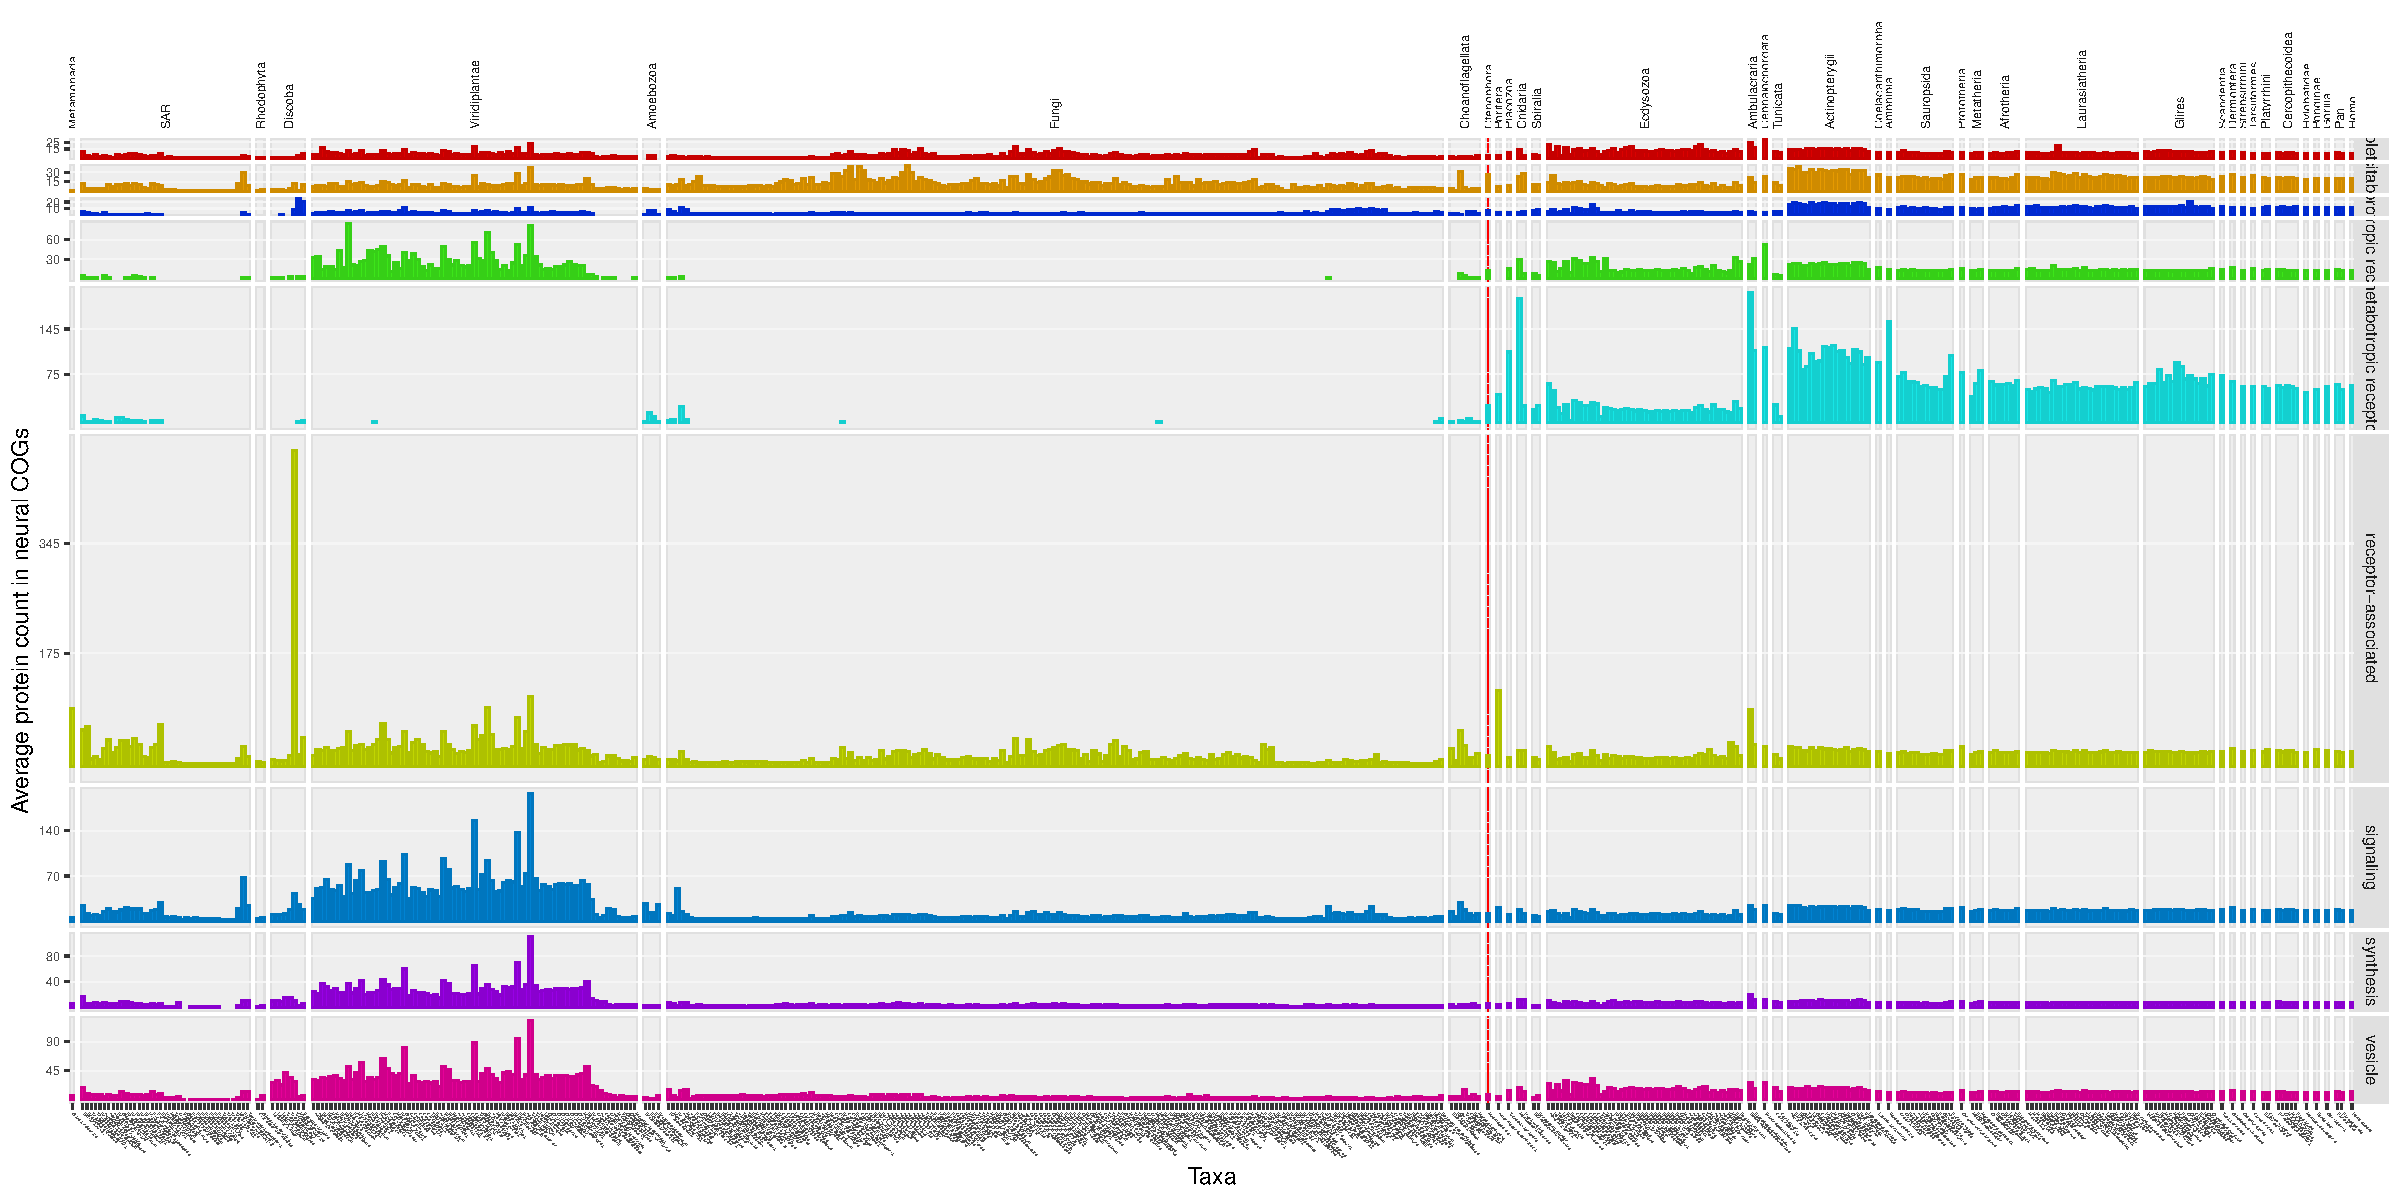
\includegraphics{figs/analysis.abundance.unnamed-chunk-5-1} 

}

\caption{A}\label{fig:unnamed-chunk-51}
\end{figure}

\begin{Shaded}
\begin{Highlighting}[]
\KeywordTok{ggsave}\NormalTok{(}\StringTok{"plots/fig5_raw.pdf"}\NormalTok{, }\DataTypeTok{width =} \DecValTok{16}\NormalTok{, }\DataTypeTok{height =} \DecValTok{8}\NormalTok{)}

\CommentTok{# Proportion --------------------}
\KeywordTok{ggplot}\NormalTok{(abundance_by_function) }\OperatorTok{+}
\StringTok{    }\NormalTok{metazoa_line }\OperatorTok{+}
\StringTok{    }\KeywordTok{geom_bar}\NormalTok{(}\KeywordTok{aes}\NormalTok{(}\DataTypeTok{x =}\NormalTok{ ncbi_name, }\DataTypeTok{y =}\NormalTok{ abundance_prop, }\DataTypeTok{fill =}\NormalTok{ annotation, }\DataTypeTok{color =}\NormalTok{ annotation), }\DataTypeTok{stat =} \StringTok{"identity"}\NormalTok{) }\OperatorTok{+}
\StringTok{    }\KeywordTok{facet_grid}\NormalTok{(annotation }\OperatorTok{~}\StringTok{ }\NormalTok{clade_name, }\DataTypeTok{scales =} \StringTok{"free"}\NormalTok{, }\DataTypeTok{space =} \StringTok{"free_x"}\NormalTok{) }\OperatorTok{+}
\StringTok{    }\KeywordTok{scale_y_continuous}\NormalTok{( }\DataTypeTok{minor_breaks =} \OtherTok{NULL}\NormalTok{) }\OperatorTok{+}
\StringTok{    }\KeywordTok{scale_fill_manual}\NormalTok{(}\DataTypeTok{values =}\NormalTok{ annotation_colors }\OperatorTok\StringTok{ }\KeywordTok{darken}\NormalTok{(}\FloatTok{0.1}\NormalTok{)) }\OperatorTok{+}
\StringTok{    }\KeywordTok{scale_color_manual}\NormalTok{(}\DataTypeTok{values =}\NormalTok{ annotation_colors }\OperatorTok\StringTok{ }\KeywordTok{darken}\NormalTok{(}\FloatTok{0.2}\NormalTok{)) }\OperatorTok{+}
\StringTok{    }\KeywordTok{theme}\NormalTok{(}
         \DataTypeTok{panel.spacing      =} \KeywordTok{unit}\NormalTok{(}\FloatTok{2.5}\NormalTok{, }\StringTok{"pt"}\NormalTok{)}
\NormalTok{        ,}\DataTypeTok{strip.background.x =} \KeywordTok{element_blank}\NormalTok{()}
\NormalTok{        ,}\DataTypeTok{strip.background.y =} \KeywordTok{element_rect}\NormalTok{(}\DataTypeTok{fill=}\StringTok{"#E0E0E0"}\NormalTok{)}
\NormalTok{        ,}\DataTypeTok{panel.grid.major.x =} \KeywordTok{element_blank}\NormalTok{()}
\NormalTok{        ,}\DataTypeTok{panel.grid.major.y =} \KeywordTok{element_line}\NormalTok{(}\DataTypeTok{colour =} \StringTok{"#F5F5F5"}\NormalTok{, }\DataTypeTok{size =} \FloatTok{0.25}\NormalTok{)}
\NormalTok{        ,}\DataTypeTok{panel.background   =} \KeywordTok{element_rect}\NormalTok{(}\DataTypeTok{fill =} \StringTok{'#EEEEEE'}\NormalTok{, }\DataTypeTok{colour =} \StringTok{'#E0E0E0'}\NormalTok{)}
\NormalTok{        ,}\DataTypeTok{strip.text.x       =} \KeywordTok{element_text}\NormalTok{(}\DataTypeTok{size =} \DecValTok{6}\NormalTok{, }\DataTypeTok{angle =} \DecValTok{90}\NormalTok{, }\DataTypeTok{hjust =} \DecValTok{0}\NormalTok{, }\DataTypeTok{vjust =} \FloatTok{0.5}\NormalTok{)}
\NormalTok{        ,}\DataTypeTok{strip.text.y       =} \KeywordTok{element_text}\NormalTok{(}\DataTypeTok{size =} \DecValTok{8}\NormalTok{, }\DataTypeTok{vjust =} \FloatTok{0.5}\NormalTok{)}
\NormalTok{        ,}\DataTypeTok{axis.text.x        =} \KeywordTok{element_text}\NormalTok{(}\DataTypeTok{size =} \DecValTok{2}\NormalTok{, }\DataTypeTok{angle =} \DecValTok{-45}\NormalTok{, }\DataTypeTok{vjust =} \DecValTok{0}\NormalTok{, }\DataTypeTok{hjust =} \DecValTok{0}\NormalTok{)}
\NormalTok{        ,}\DataTypeTok{axis.text.y        =} \KeywordTok{element_text}\NormalTok{(}\DataTypeTok{size =} \DecValTok{6}\NormalTok{)}
\NormalTok{        ,}\DataTypeTok{axis.ticks.x       =} \KeywordTok{element_line}\NormalTok{(}\DataTypeTok{size =} \FloatTok{0.1}\NormalTok{)}
\NormalTok{        ,}\DataTypeTok{legend.position    =} \StringTok{"none"}
\NormalTok{    )}
\end{Highlighting}
\end{Shaded}

\begin{figure}

{\centering 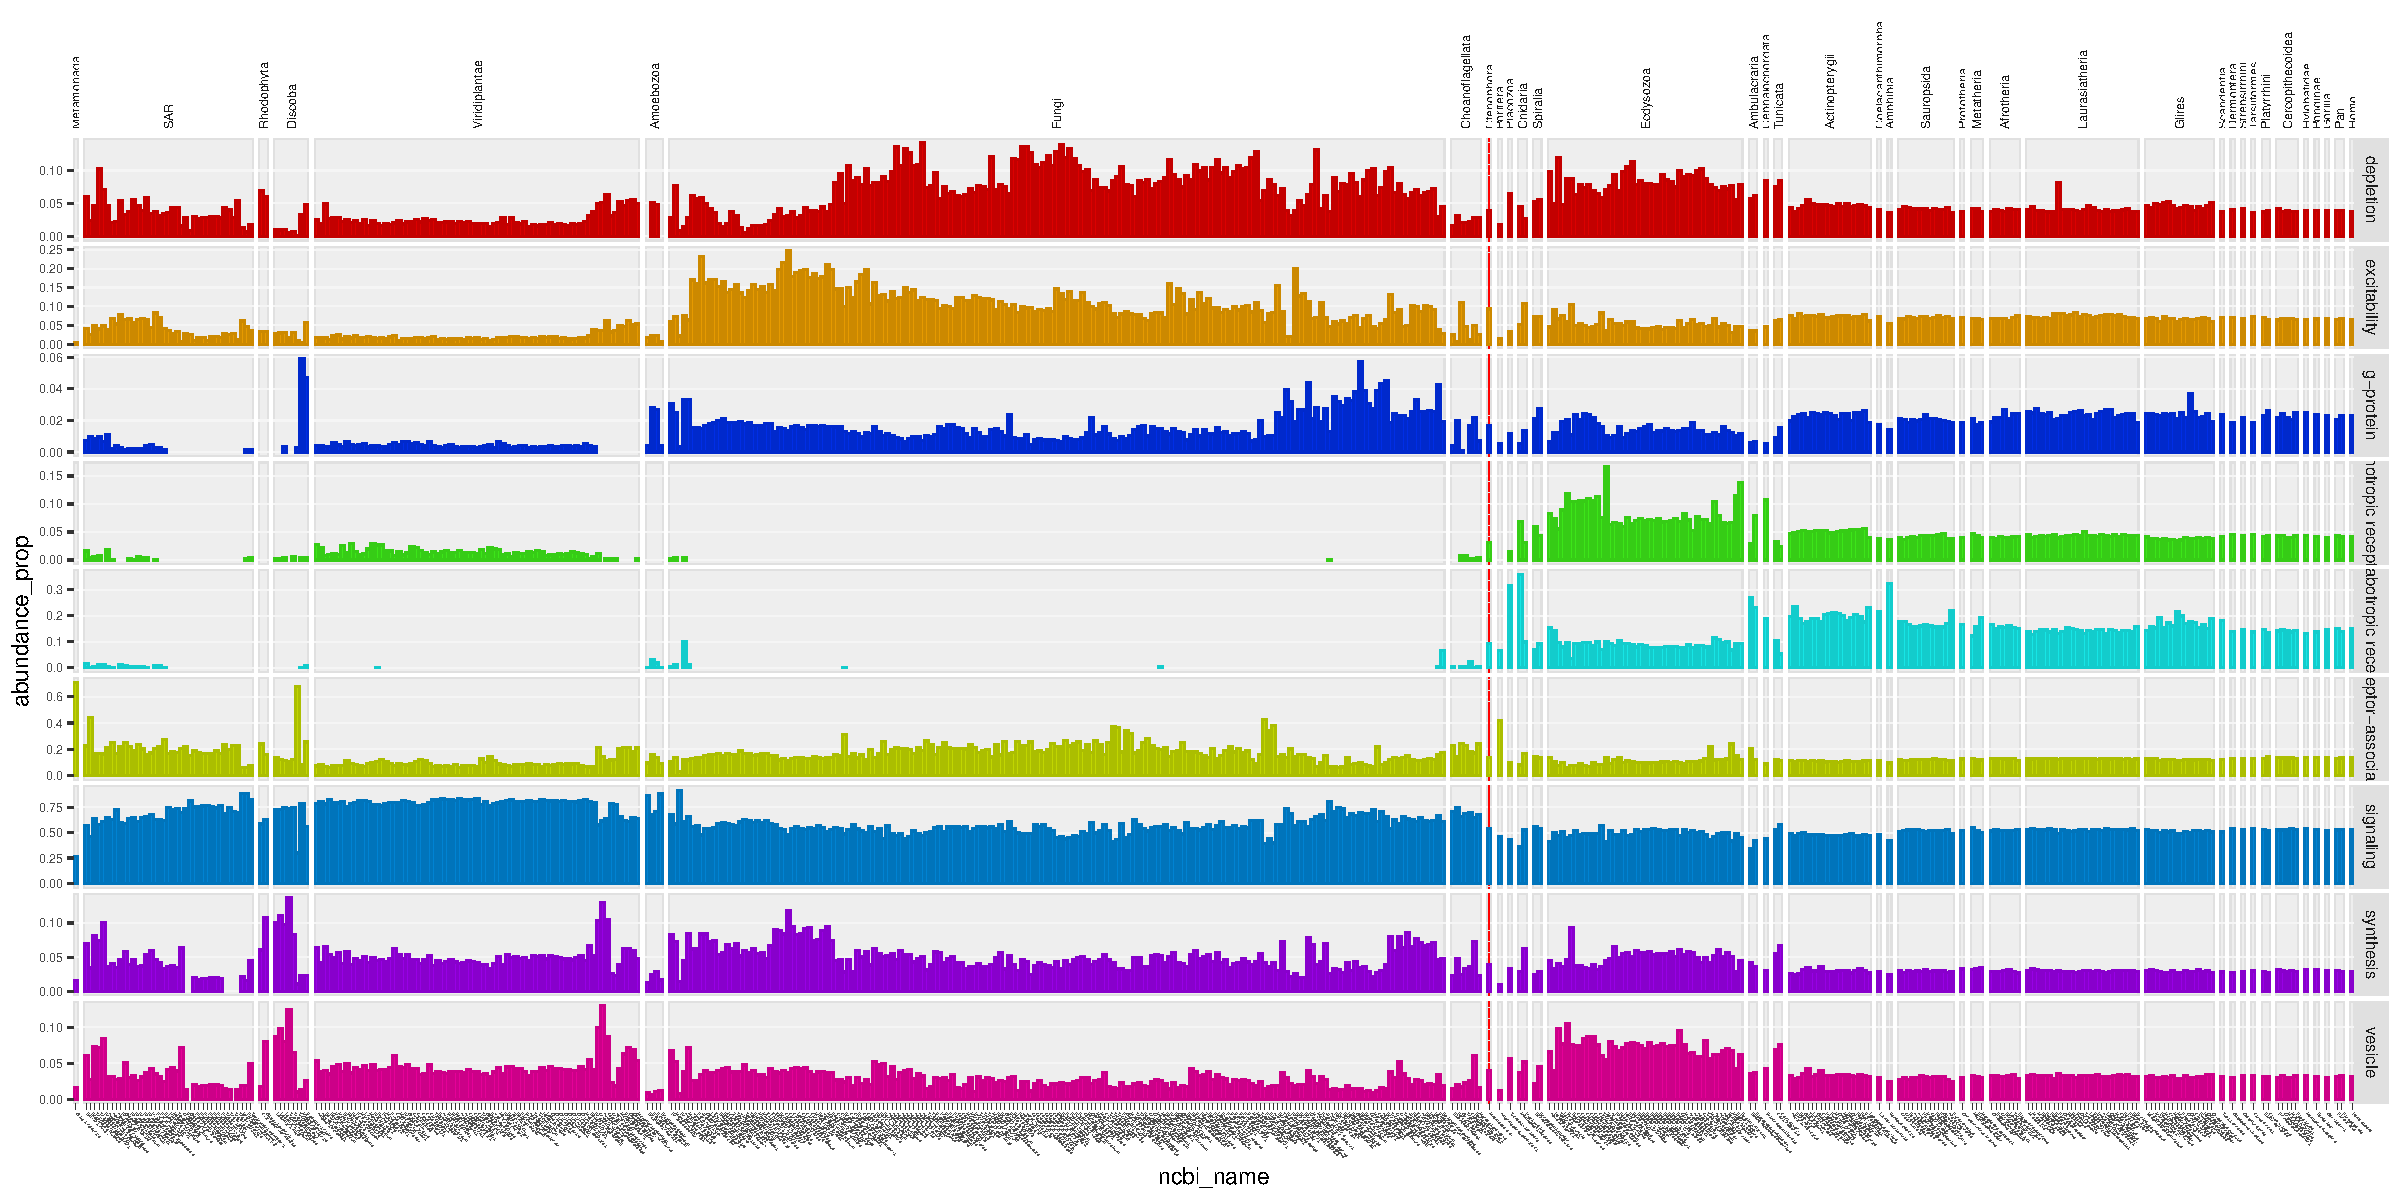
\includegraphics{figs/analysis.abundance.unnamed-chunk-5-2} 

}

\caption{A}\label{fig:unnamed-chunk-52}
\end{figure}

\begin{Shaded}
\begin{Highlighting}[]
\KeywordTok{ggsave}\NormalTok{(}\StringTok{"plots/fig5_prop_raw.pdf"}\NormalTok{, }\DataTypeTok{width =} \DecValTok{16}\NormalTok{, }\DataTypeTok{height =} \DecValTok{8}\NormalTok{)}
\end{Highlighting}
\end{Shaded}

A

\begin{Shaded}
\begin{Highlighting}[]
\KeywordTok{ggplot}\NormalTok{(abundance_by_function) }\OperatorTok{+}
\StringTok{  }\KeywordTok{geom_bar}\NormalTok{(}\KeywordTok{aes}\NormalTok{(}\DataTypeTok{x =}\NormalTok{ clade_name, }\DataTypeTok{y =}\NormalTok{ abundance, }\DataTypeTok{fill =}\NormalTok{ annotation), }\DataTypeTok{stat=}\StringTok{"summary"}\NormalTok{, }\DataTypeTok{fun =} \StringTok{"mean"}\NormalTok{) }\OperatorTok{+}
\StringTok{  }\KeywordTok{scale_fill_manual}\NormalTok{(}\DataTypeTok{values =}\NormalTok{ annotation_colors, }\DataTypeTok{guide =} \StringTok{"none"}\NormalTok{) }\OperatorTok{+}
\StringTok{  }\KeywordTok{facet_grid}\NormalTok{(annotation }\OperatorTok{~}\StringTok{ }\NormalTok{., }\DataTypeTok{scales =} \StringTok{"free"}\NormalTok{) }\OperatorTok{+}
\StringTok{  }\KeywordTok{theme}\NormalTok{(}
     \DataTypeTok{panel.spacing      =} \KeywordTok{unit}\NormalTok{(}\DecValTok{1}\NormalTok{, }\StringTok{"pt"}\NormalTok{)}
\NormalTok{    ,}\DataTypeTok{strip.text.y       =} \KeywordTok{element_text}\NormalTok{(}\DataTypeTok{angle =} \DecValTok{0}\NormalTok{, }\DataTypeTok{hjust =} \DecValTok{0}\NormalTok{)}
\NormalTok{    ,}\DataTypeTok{axis.text.x        =} \KeywordTok{element_text}\NormalTok{(}\DataTypeTok{size =} \DecValTok{5}\NormalTok{, }\DataTypeTok{angle =} \DecValTok{-45}\NormalTok{, }\DataTypeTok{vjust =} \DecValTok{0}\NormalTok{, }\DataTypeTok{hjust =} \DecValTok{0}\NormalTok{)}
\NormalTok{    ,}\DataTypeTok{axis.text.y        =} \KeywordTok{element_text}\NormalTok{(}\DataTypeTok{size =} \DecValTok{5}\NormalTok{)}
\NormalTok{  )}
\end{Highlighting}
\end{Shaded}

\begin{figure}

{\centering 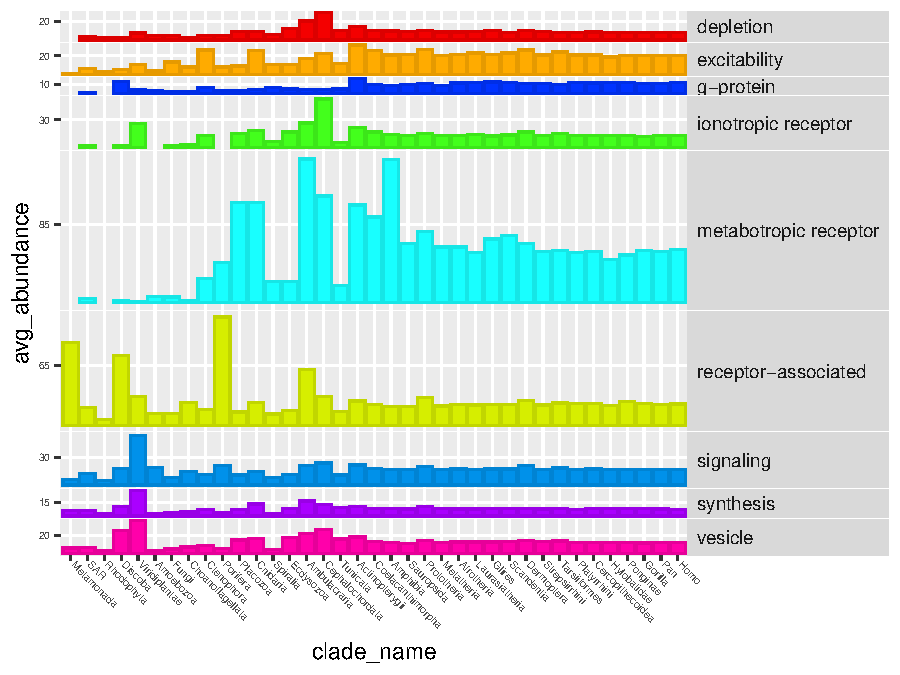
\includegraphics{figs/analysis.abundance.unnamed-chunk-6-1} 

}

\caption{A}\label{fig:unnamed-chunk-6}
\end{figure}

A

\begin{Shaded}
\begin{Highlighting}[]
\CommentTok{# Merging mixed COG functions}
\NormalTok{cog_annotation_collapsed <-}\StringTok{ }\NormalTok{cog_annotation }\OperatorTok
\StringTok{  }\KeywordTok{group_by}\NormalTok{(cog_id) }\OperatorTok
\StringTok{  }\KeywordTok{summarise}\NormalTok{(}\DataTypeTok{annotation =} \KeywordTok{paste}\NormalTok{(annotation, }\DataTypeTok{collapse =} \StringTok{"/"}\NormalTok{))}

\CommentTok{# Adding colors for mixed COGs}
\NormalTok{annotation_colors }\OperatorTok\StringTok{ }\KeywordTok{c}\NormalTok{(}
   \StringTok{"vesicle/synthesis"}\NormalTok{      =}\StringTok{ "#808080"}
\NormalTok{  ,}\StringTok{"depletion/vesicle"}\NormalTok{      =}\StringTok{ "#808080"}
\NormalTok{  ,}\StringTok{"signaling/excitability"}\NormalTok{ =}\StringTok{ "#808080"}
\NormalTok{)}

\NormalTok{protein_count_by_cog <-}\StringTok{ }\NormalTok{cog_size_by_taxid }\OperatorTok
\StringTok{  }\KeywordTok{inner_join}\NormalTok{(cog_annotation_collapsed) }\OperatorTok
\StringTok{  }\KeywordTok{left_join}\NormalTok{(ordered_species) }\OperatorTok
\StringTok{  }\KeywordTok{arrange}\NormalTok{(annotation) }\OperatorTok
\StringTok{  }\KeywordTok{mutate}\NormalTok{(}\DataTypeTok{cog_id =} \KeywordTok{fct_inorder}\NormalTok{(cog_id))}

\KeywordTok{ggplot}\NormalTok{(protein_count_by_cog) }\OperatorTok{+}
\StringTok{  }\NormalTok{metazoa_line }\OperatorTok{+}\StringTok{ }
\StringTok{  }\KeywordTok{geom_bar}\NormalTok{(}\KeywordTok{aes}\NormalTok{(}\DataTypeTok{x =}\NormalTok{ ncbi_name, }\DataTypeTok{y =}\NormalTok{ cog_size, }\DataTypeTok{fill =}\NormalTok{ annotation), }\DataTypeTok{stat =} \StringTok{"identity"}\NormalTok{) }\OperatorTok{+}
\StringTok{  }\KeywordTok{scale_fill_manual}\NormalTok{(}\DataTypeTok{values =}\NormalTok{ annotation_colors }\OperatorTok\StringTok{ }\KeywordTok{darken}\NormalTok{(}\FloatTok{0.2}\NormalTok{), }\DataTypeTok{guide =} \StringTok{"none"}\NormalTok{) }\OperatorTok{+}
\StringTok{  }\KeywordTok{scale_y_continuous}\NormalTok{(}\DataTypeTok{breaks =} \KeywordTok{tick_function}\NormalTok{(}\DecValTok{3}\NormalTok{, }\DecValTok{1}\NormalTok{), }\DataTypeTok{minor_breaks =} \OtherTok{NULL}\NormalTok{) }\OperatorTok{+}
\StringTok{  }\KeywordTok{facet_grid}\NormalTok{(cog_id }\OperatorTok{~}\StringTok{ }\NormalTok{., }\DataTypeTok{scales =} \StringTok{"free_y"}\NormalTok{) }\OperatorTok{+}
\StringTok{  }\KeywordTok{theme}\NormalTok{(}
     \DataTypeTok{panel.spacing      =} \KeywordTok{unit}\NormalTok{(}\FloatTok{0.5}\NormalTok{, }\StringTok{"pt"}\NormalTok{)}
\NormalTok{    ,}\DataTypeTok{panel.grid.major.x =} \KeywordTok{element_blank}\NormalTok{()}
\NormalTok{    ,}\DataTypeTok{panel.grid.major.y =} \KeywordTok{element_line}\NormalTok{(}\DataTypeTok{size =} \FloatTok{0.1}\NormalTok{, }\DataTypeTok{linetype =} \StringTok{"dashed"}\NormalTok{)}
\NormalTok{    ,}\DataTypeTok{strip.text.y       =} \KeywordTok{element_text}\NormalTok{(}\DataTypeTok{size =} \DecValTok{4}\NormalTok{, }\DataTypeTok{angle =} \DecValTok{0}\NormalTok{, }\DataTypeTok{hjust =} \DecValTok{0}\NormalTok{)}
\NormalTok{    ,}\DataTypeTok{axis.text.x        =} \KeywordTok{element_text}\NormalTok{(}\DataTypeTok{size =} \FloatTok{1.5}\NormalTok{, }\DataTypeTok{angle =} \DecValTok{-45}\NormalTok{, }\DataTypeTok{vjust =} \DecValTok{0}\NormalTok{, }\DataTypeTok{hjust =} \DecValTok{0}\NormalTok{)}
\NormalTok{    ,}\DataTypeTok{axis.text.y        =} \KeywordTok{element_text}\NormalTok{(}\DataTypeTok{size =} \DecValTok{4}\NormalTok{)}
\NormalTok{    ,}\DataTypeTok{axis.ticks         =} \KeywordTok{element_line}\NormalTok{(}\DataTypeTok{size =} \FloatTok{0.1}\NormalTok{)}
\NormalTok{  )}
\end{Highlighting}
\end{Shaded}

\begin{figure}

{\centering 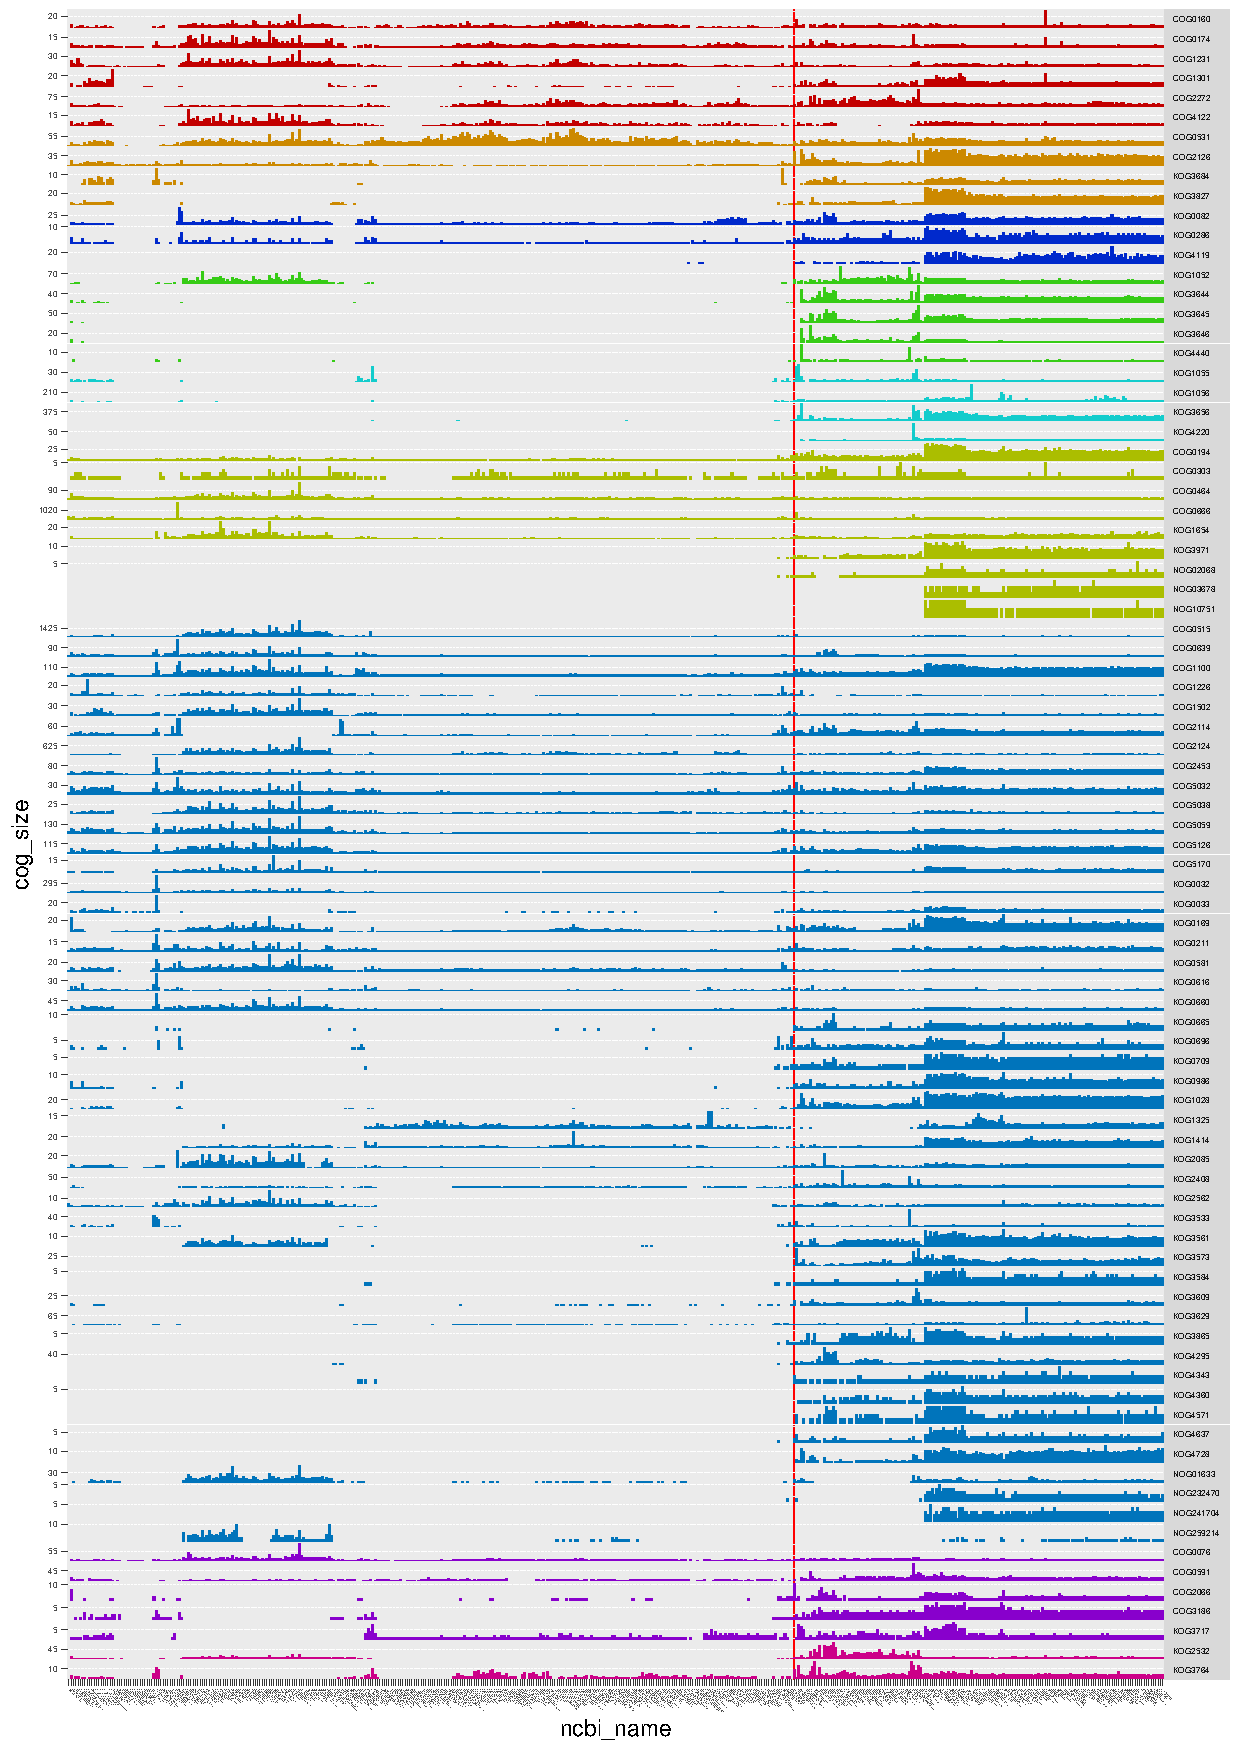
\includegraphics{figs/analysis.abundance.unnamed-chunk-7-1} 

}

\caption{A}\label{fig:unnamed-chunk-7}
\end{figure}
